\newpage
\section{Symmetric abstractions}\label{symmetric-abstractions}

% symmetry is cool
Symmetry is a concept from pure mathematics, which has found major success in physics ref ref ref.
(why has it found such success in physics? beauty, compression, ... Occam's razor)

Recently, it has also been applied in machine learning in some imortant ways; to disentanglement \cite{Higgins2018} which makes a lot of sense because ...,
% Connection to causal hierarchy. Cite Pearl. Association, intervention, counterfactuals.
Also recently noted by \cite{Caselles-Dupre2019}, ... where they assume that
the group actions are the actions of the RL environment.
This doesn't really make sense. Also, will miss many symmetries like ???

% occam's razor
Occam's razor is a core idea behind much of statistics, ML and science. Simple
hypotheses should be preferred as the are more likely to be right.
% This intuition can be viewed a little more formally through a Bayesian perspective.

% symmetry and occams razor
How does symmetry relate to simplicity?

\subsubsection{Definition}

A say that an object is symmetric is it has a 'group' structure.

A group is a set, $G$ (\textit{say the set of rotations, $\{0, 90, 180, 270\}$}),
and an operation $\circ$ that combines any two elements $a$ and $b$ to form
another element (\textit{rot $90$ composed with rot $180$ is rot $270$, or} $a \circ b = a + b \;\text{mod} 360$).
To qualify as a group, the set and operation, $(G, \circ)$, must satisfy four requirements;

\begin{itemize}
	\tightlist
	\item \textbf{Closure:} For all $a, b \in G$, the result of the operation $a \circ b$ is also in $G$. (\textit{every composition of two rotations, must also be a rotation})
	\item \textbf{Associativity:} For all $a,b,c \in G$, $(a\circ b) \circ c = a\circ (b\circ c)$. (\textit{???})
	\item \textbf{Identity element:} There exists and element $e\in G$ such that, for every element $a\in G$, the equation $e\circ a = a\circ e = a$ holds. (\textit{there must exist a rotation that doesn't rotate})
	\item \textbf{Inverse element:} For each $a \in G$, there exists an element $b \in G$, commonly denoted $a^{−1}$, such that $a \circ b = b \circ a = e$. (\textit{we must be able to undo any rotation})
\end{itemize}

For example, we can imagine the \textit{action} of this rotation group $\big(0, 90, 180, 270, \circ \big)$ on a playing card. (bad example!?)

\begin{figure}[h!]
	\centering
	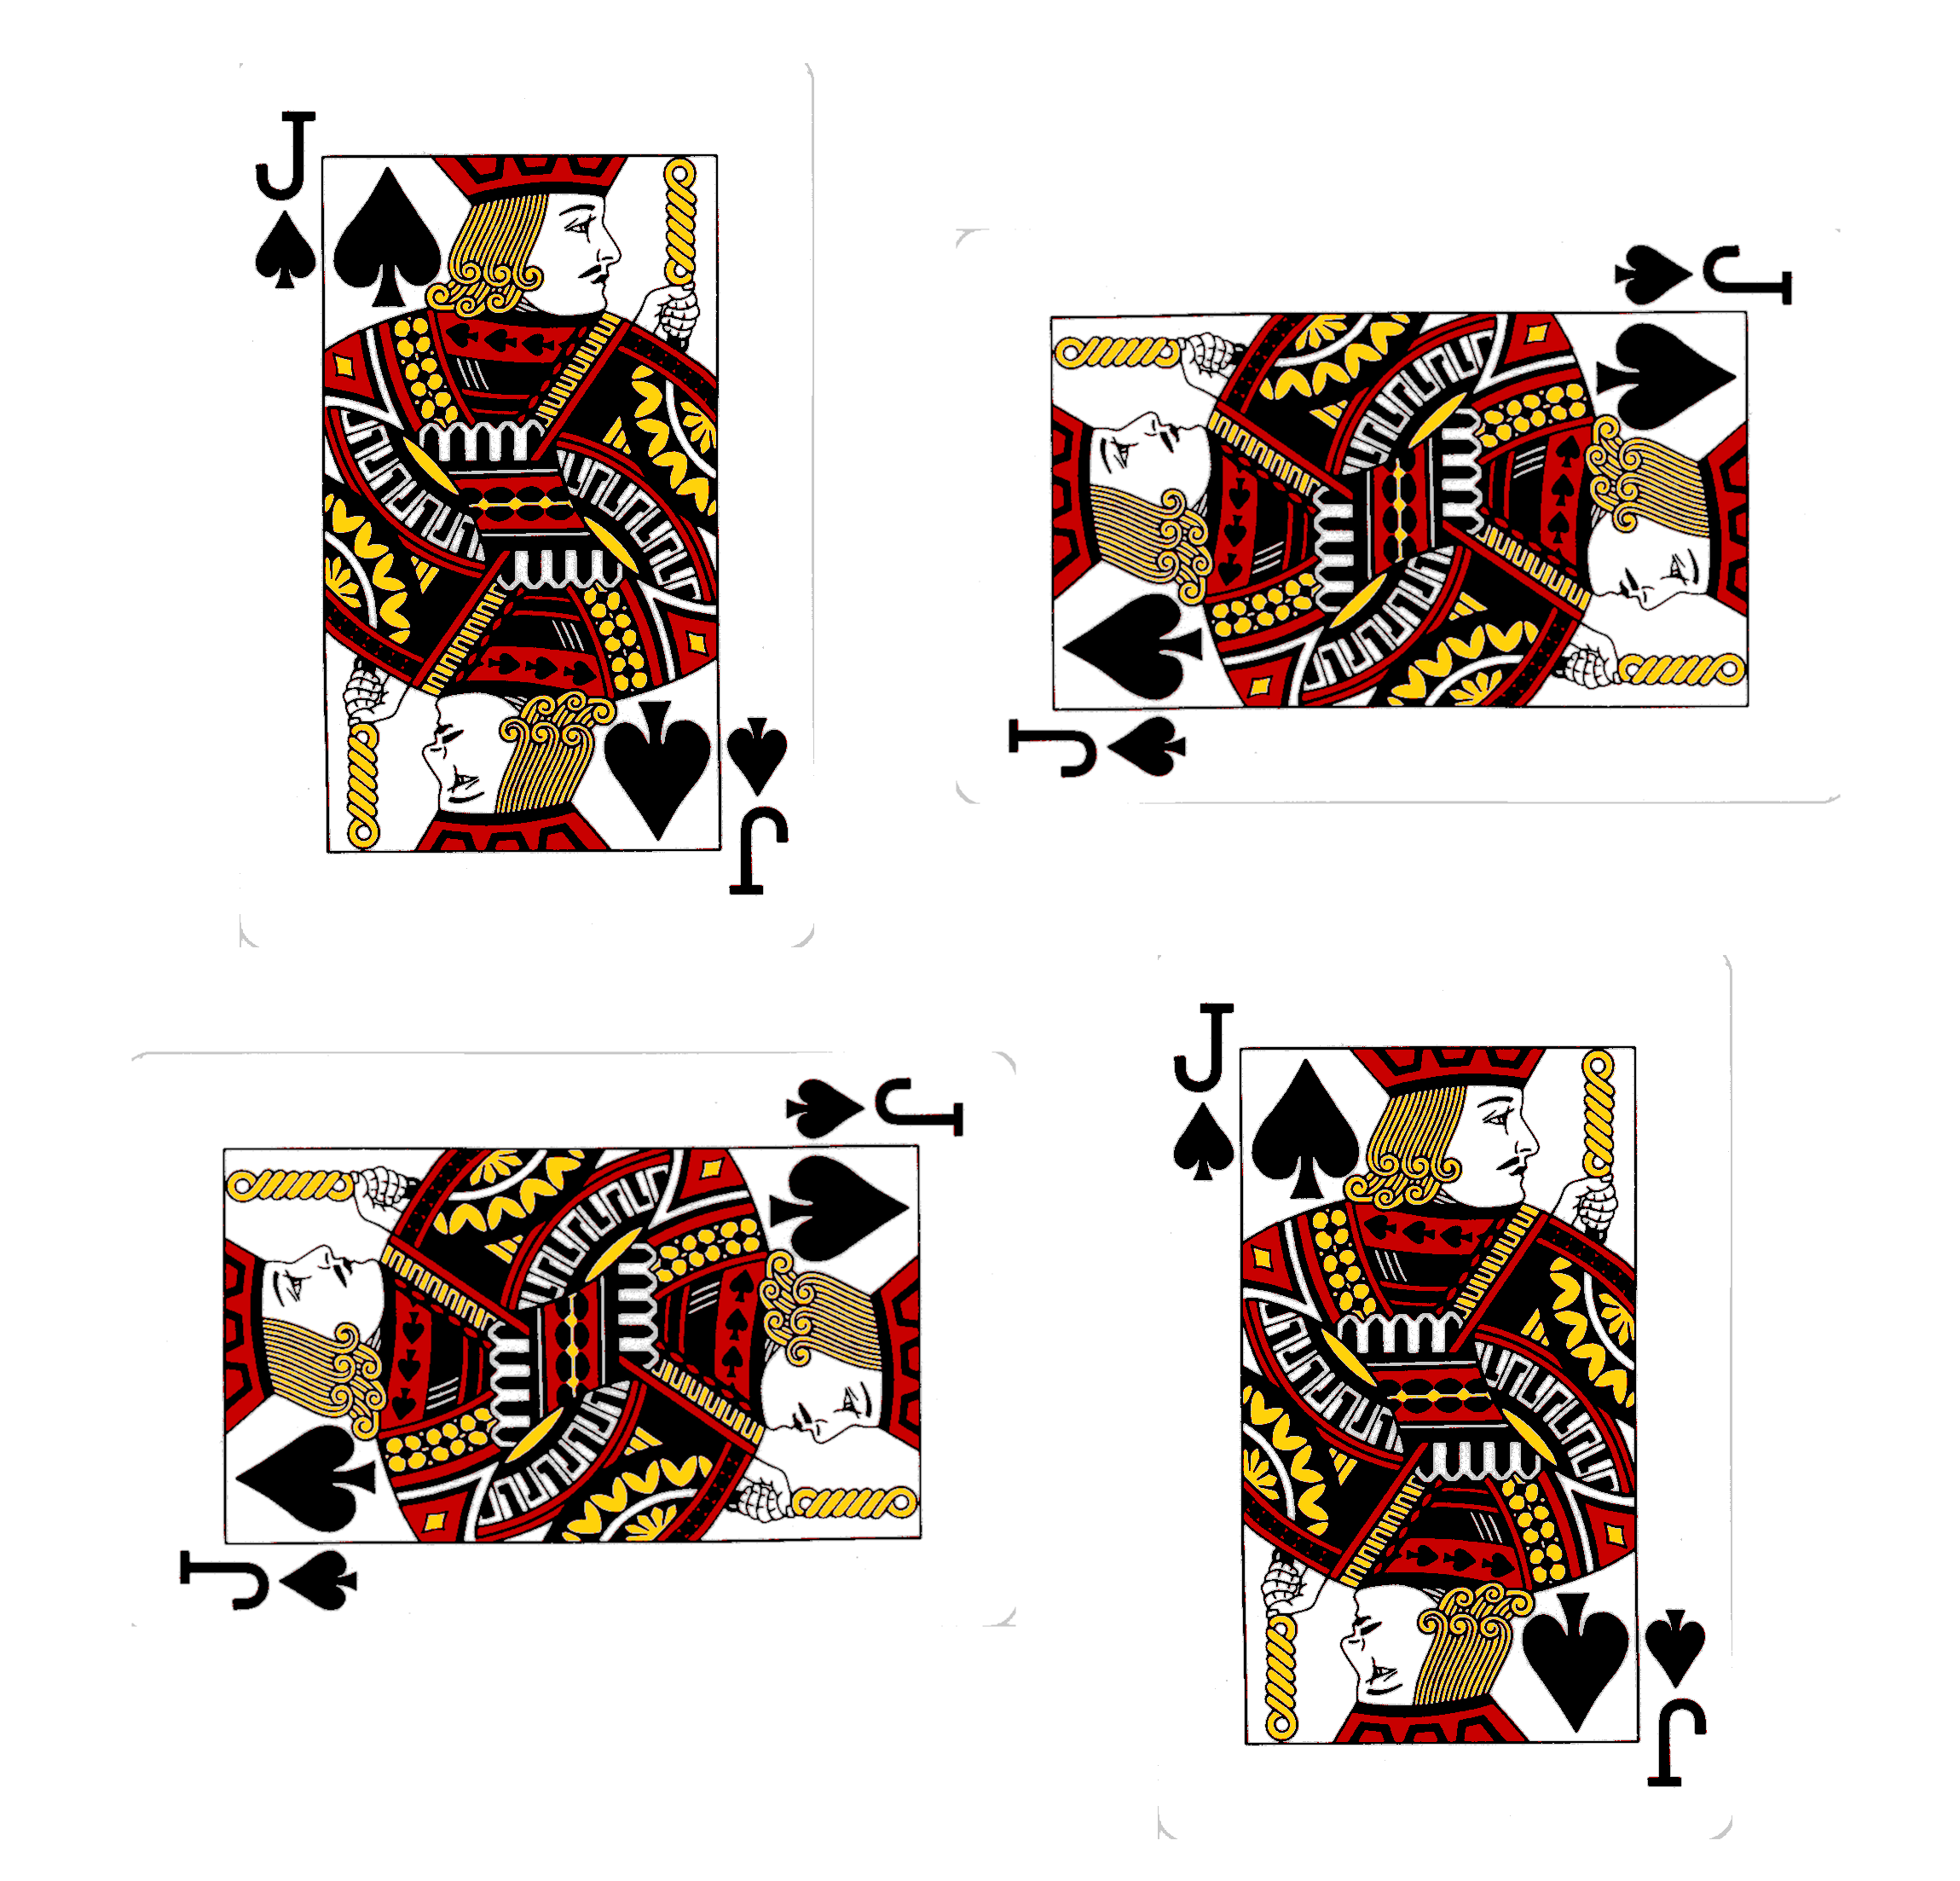
\includegraphics[width=0.75\textwidth,height=0.5\textheight]{../../pictures/images/jacks.png}
	\caption{Here we have applied the group of four rotations to a Jack of spades.
	However, we see that there exists symmetry within the these rotations,
	there are only two distinct rotations, vertical and horizontal. This is because }
\end{figure}

The action of a group on XXX.

\subsubsection{Symmetries and abstractions}

\begin{displayquote}
\textsl{How do symmetries help us build abstractions?}
\end{displayquote}

We can use a group structure to define a similarity (or equivalence relation),
$a \sim_G b$ iff $\exists g \in G: a = g \circ b$. {\color{red} for example??} Therefore, we can use this
 notion of similarity to construct abstractions as we did in \ref{C:abstraction}.

 \subsubsection{A symmetric inductive bias}

 % This is about generalising using an inductive bias towards symmetry.

 In the introduction to abstractions for RL we considered learning similarities
 to build an abstraction. But, learning pairwise similarities does not give
 you the ability to generalise. To generalise you need priors. For example;
 CNNs generalise because they implicitly encode priors for smoothness and explicitly for locality. (ref)

 Another potentially useful prior is symmetry: \textit{"We believe it is likely that
 the problems we are given have some symmetry within them."}

 The intuition is, this symmetry prior helps us generalise because, we can guess
 a symmetry that matches the observed pairwise similarities. This symmetry might
 require that other pairs to be similar (because of the closed natured of groups).
 Thus, we can generalise knowledge from some pairwise similarities to others
 pairwise similarities (assuming the prior is correct).


 \begin{center}\rule{0.5\linewidth}{\linethickness}\end{center}


 Symmetry is a stricter notion of similarity.
 If $x, x' \in X$ are symmetric, then there must exist $f$ such that $f(x) = x'$.
 Where, $(X, f)$ must satisfy the group axioms, (closure, associativity, identity, inverse).

 The key property we are interested in is closure.
 Two $x, x'$ are considered symmetric if $\exists g\in G$


 How can it be discovered?

 A couple parts. Discovery of symmetries, exploration of the knowledge of symmetries.

 Unsupervised discovery. Not much success yet. Only when using some kind of supervised signal.

 \cite{Ho2019a, Lim2019, Cubuk2018, Cubuk2019}
 Discover which symmetries apply to a given domain, and at what magnitude.
 The optimisation problem becomes one of picking the probability of each op and its magnitude.
 There is a small set of ops (aka symmetries) that are given:
 \textit{Identity, AutoContrast, Equalize, Rotate, Solarize, Color, Posterize, Contrast,
 	Brightness, Sharpness, ShearX, ShearY, TranslateX, TranslateY.}
 Uses validation error as a reward for learning.

 \subsubsection{Inferring symmetries from experience}

 % How easy is it to solve this symmetry inference problem?

 % HOW?!

 What does this buy us? If have sufficient data to tell us that $x$ and $y$ are
 similar, say that they are mirror images of each other.
 As an unsupervised pre-training step. Then apply and share labels and learn more quickly?
 What else can $x$ tell us about $y$?

 \cite{Yang2019}

 Or end to end? As we get more certain that x and y are similar, we more strongly
 encourage their symmetry through one of the methods outlined above.
 Is it possible (/easier) to learn that x and y are similar (in terms of their labels) before (accurately) learning their labels.



 Want to have an inductive bias towards simpler symmetries. But, how can we do this without needing to represent all possible symmetries?
 A solution rejection sampling??


 % - What about symmetries that are products of subgroups? $S = Z_2 \times Z_3$? Are they easier to infer?
 % - Within the same $n$. Is there a notion of more or less complex group structures??
 % - Need to show that NNs dont have the right symmetric inductive bias. They dont generalise. !!!

 % Examples

 % - Knowing that; range $= [0,360)$, and $0, 45, 90, 135, 180$, all are similar. I guess that we are in cyclic group $8$ and therefore $225, 270, 315$ are also similar. Key is that I know that $0, 45, 90, 135, 180$ are related by $0+0, 0+45, 0+45+45, 0+45+45+45, 0+45+45+45+45$.
 % - Cart pole. $V^{\pi(s, a)}(s') = V^{\pi(-s, -a)}(-s') \forall s'$.

 If we know the order of the group, then how hard is the problem?
 For many (lower) orders, there is only one or two possible symmetries. http://mathworld.wolfram.com/FiniteGroup.html

\subsection{Symmetries for RL}\label{mdp-homomorphism}

Different ways to approach characterising symmetries; automorphisms, invariants relations.
% how do these two relate!?

\subsubsection{Automorphisms}

Closely related to a homomorphism. See for a definition of a MDP homomorphism that captures symmetries.
% As pointed out in \ref{abstraction}, the notion of an abstraction is captured by a homomorphism.
% So, what would it look like if we had a MDP homomorphism?

\cite{Ravindran2002}

$\mathcal H: \mathcal M\to \mathcal M$.

\begin{align}
P(f(s')|f(s), g_s(a)) = \sum_{s''\in [s']_f} P(s''| a, s) \\
r(f(s), g_s(a)) = r(s, a)
\end{align}

This MDP homomorphism framework is a state-action abstraction, that uses a model based notion of similarity.
However, as pointed out in eariler sections, there are many other possible
notions of abstraction and similarity that make sense for RL. Specifically, the MDP homomorphism framework
could be generalised in the following ways;

\begin{itemize}
\tightlist
  \item temporal symmetries
  \item approximate symmetries
  \item inference of symmetries under uncertainty
  \item complexity measure / inductive bias
\end{itemize}

\subsubsection{Invariants}

While there are many types of finite group, (cyclic, alternating, ...?) And then there are continuious symmetries, (Lie groups)
Which types of symmetry are important for RL problems?

Let's work through an example, the cart-pole control problem. Your goal is to balance a pole on a cart.
You are allowed to move the cart left or right.

% How hard is it to find these symmetries?
% Are some harder than others?

\begin{figure}[h!]
	\centering
	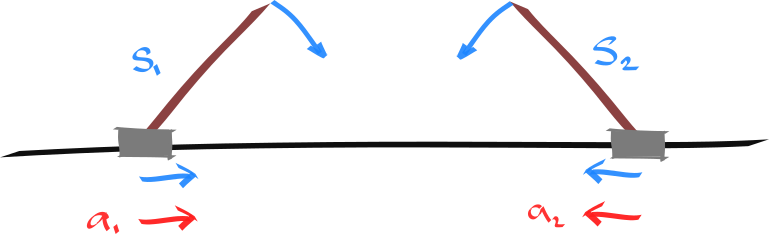
\includegraphics[width=1\textwidth,height=0.25\textheight]{../../pictures/drawings/cart-pole-mirror.png}
	\caption{Two mirror symmetric states of a cart pole. But in what sense are they symmetric?}
\end{figure}

% Need to show this is actually a symmetry, isomorphic to $S_2$?!?
In the case above, the mirrored cart pole is an instance of $S_2$.
The action $f, g$ we apply to the MDP is isomorphism to the simple finite group, $S_2$

Symmetries can be uniquely characterised by their invariants \cite{PeterOlver1999}.
What are the interesting invariants of MDPs? And how do they ???
But, what does this symmetry imply about other quantities of interest for RL?

Invariance, $f(g(x)) = f(x)$, equivariance, $f(g(x)) = g(f(x))$.

In general we want to know;

\begin{itemize}
	\tightlist
	\item We have $n$ different 'symmetries'. But are they really different?
	\item Which symmetries share some invariants?
	\item Which invariants uniquely characterise this symmetry?
\end{itemize}

With this knowledge, we could identify symmetries via their invariants!?!
We can observe invariant properties. (not clear to me how you observe a symmetry!?)

We briefly explore this in \ref{game-invariants}.

\subsubsection{Exploitation} \label{symmetric-exploitation}

\begin{displayquote}
\textsl{Once have discovered a symmetry, how might we exploit that knowledge?}
\end{displayquote}

Similar to how we considered how to exploit an abstraction in section \ref{},
let's review some existing methods for exploiting the knowledge of a symmetry. \footnotemark[22]

\footnotetext[22]{Note that, in all of these methods, symmetry provides
advantage over considering just the pairwise similarities. We will return to this later.}

% note: what has been given to these methods of exploitation?
% knowledge of the group, or its actions, or ...?

\paragraph{Exploiting symmetry for efficient control}

If we have a MDP, $M_1$, then solving it via value iteration requires $\mathcal O(\epsilon |S|^2|A|)$ iterations.
However, if we know that there exists symmetries in the state space, then we can 'minimise the model',
by applying the MDP homomorphism $\mathcal H: \mathcal M\to \mathcal M$.
This new, minimised, MDP, $M_2$ has a smaller state space, as $|S_{M_2}| = \frac{|S_{M_1}|}{k}$
and essentially the same dynamics and rewards. Thus we can solve $M_2$, with cost $\mathcal O(\epsilon \frac{|S|^2|A|}{k^2})$
and then lift the solution back to $M_1$. \cite{Dean1997, NARAYANAMURTHY}


\paragraph{Exploiting symmetry for efficient inference}

There has been a large amount of work (that we are familiar with) exploring
the exploitation of ... See  here for an overview \ref{symmetry-inference}.

The general essence of the idea is \textit{"invariance reduces variance"}. \cite{Chen2019}

Locomotion sharing ... \cite{Abdolhosseini}

By sharing weights according to group structure\cite{Ravanbakhsh2017a}, we can increase the effective data seen by each weight.

\paragraph{Exploiting symmetry for efficient exploration}

Holtzen et al. \cite{Holtzen2019} show that by grouping together variables according to
the knowledge of a symmetry, they show that \textit{orbit-jump MCMC mixes rapidly in the number of orbits}.
In other words, symmetries allow the efficient estimation of distributions.
% Want to demonstrate this.
% {\color{red}TODO max ent + abstraction experiments}

Also. \cite{Campbell2019}

\begin{center}\rule{0.5\linewidth}{\linethickness}\end{center}

All of these methods rely on a similar type of argument. Picking a representative
of a partition and only using that one. Averaging over orbits. ...

\subsection{Symmetry measure}

To discover symmetries, we need to be able to measure them. Using this measure, we can

\begin{align*}
C(x) = \mathop{\text{min}}_y S(y) + E(x, y)
\end{align*}

Need to;

\begin{itemize}
	\tightlist
	\item Construct a symmetry measure $S: Y \to \mathbb R^+$
	\item Find a way to efficiently search through $Y$.
	\item Pick a $E(x, y^{* })$.
	\item Use $C(x)$ to accelerate learning (/ get money).
\end{itemize}

\subsubsection{Complexity of symmetries}

Desiderata of complexity measure;

\begin{itemize}
	\tightlist
	\item $\mathcal L(C_4) > \mathcal L(C_2 \oplus C_2)$
	\item $\mathcal L(D_4) > C_8$ (because $D_4$ is not abelian)
	\item A perfect symmetry should have lower complexity than $C([a,a,b,c]) < C([a,a+\epsilon,b,c])$
	\item Symmetries with larger ??? should have lower complexity. $C([a,b,a,b]) < C([a,a,b,c])$
	\item $C([a,a,b,c]) = C(10 \times [a,a,b,c])$
\end{itemize}

% What about characterising the complexity by the number of generators /relations.
% Or something information theoretic?

We restrict the familiy of symmetries to $S_2$ $C(x) = E(x, y^{* })$ to accelerate learning.
Next, we condider need to construct

Not explicit knowledge of a symmetry. But, a family of symmetries. A higher level prior.

Future work. Generalise to more symmetries.

% \begin{align*}
% C(x) = -\log \sum_{y\in Y} e^{-S(y) - E(x, y)}
% \end{align*}

\begin{align*}
C(x) &= \mathop{\text{argmax}}_i  \parallel x-P_i\cdot x\parallel_2 + e^{-S(P_i)^2}\\
\end{align*}

\subsubsection{Topology}

\begin{figure}[h!]
\centering
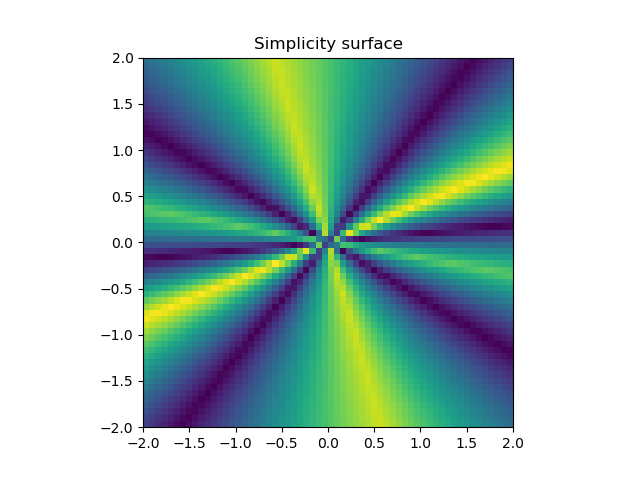
\includegraphics[width=1\textwidth,height=0.5\textheight]{../../pictures/figures/complexity_surface_nd-3d.png}
\caption{}
\end{figure}

\begin{figure}[h!]
\centering
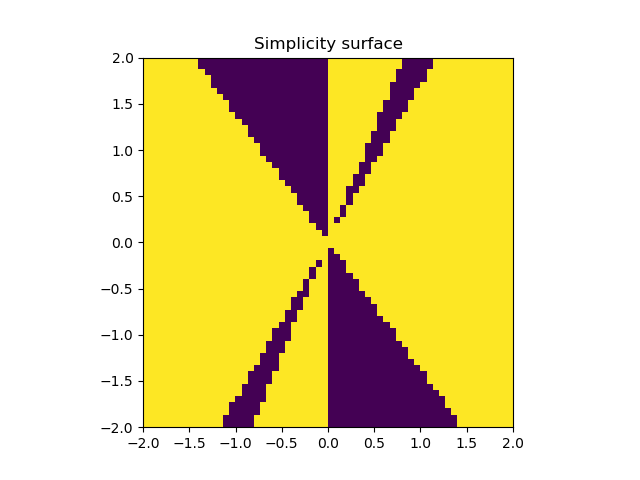
\includegraphics[width=1\textwidth,height=0.5\textheight]{../../pictures/figures/complexity_surface_nd-4d-S-0.png}
\caption{}
\end{figure}

\begin{figure}[h!]
\centering
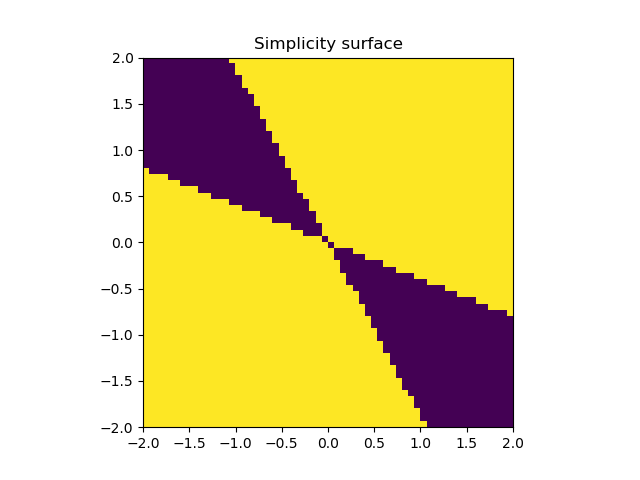
\includegraphics[width=1\textwidth,height=0.5\textheight]{../../pictures/figures/complexity_surface_nd-4d-S-2.png}
\caption{}
\end{figure}

\subsubsection{Scalability}

Increases quickly. 2->1, 3->3, 4->9, 5->25, 6->75, 7->231, 8->763, 9->??

\begin{figure}[h!]
\centering
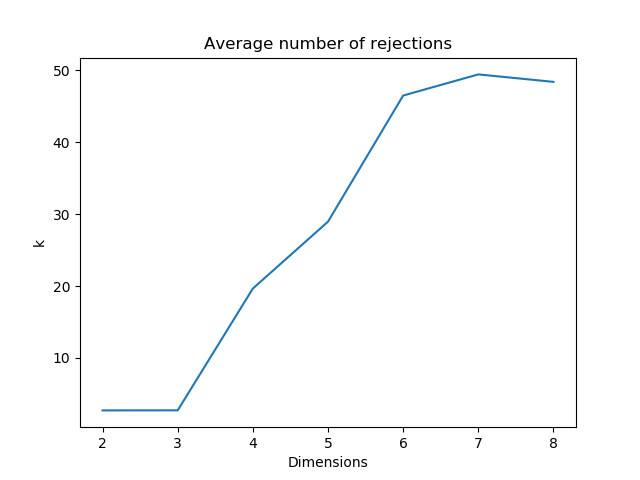
\includegraphics[width=1\textwidth,height=0.5\textheight]{../../pictures/figures/ks.png}
\caption{}
\end{figure}


Why so expensive? There is no structure in the states. They are discrete and unrelated.
(at least our representation of them). Cyclic symmetry is easy to detect in (example) because
we ... .


\subsection{Biased Thompson Sampling} \label{thompson-sampling}

Following our insights from \ref{symmetry} and \ref{???}.

% A way to add explicit inductive biases is via importance (/ rejection) sampling.

% Most general way of adding a prior!?!? Doesnt assume that SGD is being done, or some parameterisation... !??!?!


\subsubsection{Thompson sampling}
\begin{displayquote}
	\textsl{What is Thompson Sampling?}
\end{displayquote}

\begin{displayquote}
	\textit{Thompson sampling is an algorithm for online decision problems where actions are taken sequentially in a manner that
must balance between exploiting what is known to maximize immediate performance and investing to accumulate
new information that may improve future performance.}\cite{Russo2017}
\end{displayquote}


\begin{algorithm}
	\caption{Thompson Sampling}
	\begin{algorithmic}[1]

		\Procedure{TS}{$\gamma$}
		\State $t=0$
		\While{not converged}
		\State $(s, a, r, s')$ \Comment{Observe}
		\State $H_t \leftarrow (s, a, r, s', a')$ \Comment{Update history}
		\State $\tau, R \sim P(\cdot | H_t)$ \Comment{Sample a model}
		\State $Q_{t+1}(s, a) = R(s, a) + \gamma \tau(s'| s, a) Q_t(s', a')$ \Comment{Bellman operator}
		\State $\pi_t = \text{greedy}(Q_{t+1})$ \Comment{Act greedily}
		\State $t += 1$

		\EndWhile
		\State \algorithmicreturn{ $\pi_t$}
		\EndProcedure

	\end{algorithmic}
\end{algorithm}

Where $H_t$ is the history of observations, $(s, a, r, s')$.
And we construct $P(\tau, R | H_t) = P(\tau | H_t) \cdot P(R | H_t)$. Where $P(\tau | H_t)$
is modelled as a non-parametric distribution: the normalised.
And $P(R | H_t)$ is modelled as a isotropic gaussian.
These can be estimated by storing state-action-state transition counts
and the incremental mean and variance of the rewards.

Note that we act greedily with respect to the $Q$ function. Normally, this would
lead to sub optimal behaviour, because no exploration is being done. But, Thompson sampling
directs exploration through its uncertainty in the model, $\tau, r$. Thus,
exploration occurs by acting greedily with respect to a sampled model.

\subsubsection{Abstracted Thompson Sampling}

There may be structure in the model,
Thompson sampling from estimates of similarity / symmetry.

The likelihood of an abstraction, $P(A|H_t)$, is modelled as a isotropic (actually should really use full covar?!?!) guassian.

\begin{align*}
	P(A|H_t) &= \mathcal N(\chi_{\mu}, \chi_{\sigma}) \\
	\chi_{\mu} &= \frac{1}{t}\sum_{i=0}^t Q_i \tag{mean} \\
	\chi_{\sigma} &= \sqrt{\sum_{i=0}^t (Q_i - \chi_{\mu})^2} \tag{standard deviation}
\end{align*}

When notice that two states are similar, we group them together. After grouping them, we can apply the Bellman optimality operator.

\begin{algorithm}
	\caption{Abstracted Thompson sampling}
	\begin{algorithmic}[1]

		\Procedure{ATS}{$\gamma$}
		\State $t=0$
		\While{not converged}
		\State $(s, a, r, s')$ \Comment{Observe}
		\State $H_t \leftarrow (s, a, r, s', a')$ \Comment{Update history}
		\State $\tau, R \sim P(\cdot | H_t)$ \Comment{Sample a model}
		\State $A \sim P(\cdot | H_t)$ \Comment{Sample a state abstraction}
		\State $\tilde \tau, \tilde r, \tilde Q_t = A(\tau, r, Q_t)$ \Comment{Do a model reduction}
		\State $\tilde Q_{t+1}(s, a) = \tilde r(s, a) + \gamma \tilde \tau(s'| s, a) \tilde Q_t(s', a')$ \Comment{Bellman operator}
		\State $Q_{t+1} = S^{-1}(\tilde Q_{t+1})$ \Comment{Lift the values}
		\State $\pi_t = \text{greedy}(Q_{t+1})$ \Comment{Act greedily}
		\State $t += 1$

		\EndWhile
		\State \algorithmicreturn{ $\pi_t$}
		\EndProcedure

	\end{algorithmic}
\end{algorithm}

% if we were certain enough, we could throw away estimates of certain states. and just work in the abstracted domain?!

This doesnt really work. For a few reasons. Costs a lot of keep track of the pairwise state similarities.
Saves compute on Bellman step.
But overall, is probably costing more compute than has been gained.

Shouldn't effect sample efficiency.

\subsubsection{Biased Abstracted Thompson Sampling}

The difference between \textit{Abstracted Thompson Sampling} and \textit{Biased Abstracted Thompson Sampling}
is how we construct the distribution over abstractions, $P(A|D)$.

We believe that the states will have group structure, a symmetry. ({\color{red}why?})
Therefore, we want a way to say: state abstractions, $A$, that are symmetric should be more likely.

To achieve this, we need to construct a distribution, $P_S(A)$, that prefers more symmetric abstractions.
We can then use this prior, with maximum a posterori, to estimate the posteror as $P(A | H_t) = \frac{P(H_t | A)P_S(A)}{P(H_t)}$.

However, there are a couple of problems. Constructing $P_S(A)$. Estimating $P(H_t)$, ...?
Actually, we dont need to construct it, we only need samples from $P(A | D)$.

See \ref{rejection-sampling}.

\begin{center}\rule{0.5\linewidth}{\linethickness}\end{center}

Assuming the prior is corrent. How much compute does it cost? And how many samples does it buy?

Need to calculate;

\begin{itemize}
	\item Computational cost of finding all the actions of $S_2$ on a d-dimensional vector.
	\item The number of rejected samples required (on average), before one is accepted. (and how this scales with $|S|$)
	\item
\end{itemize}

% This solves the efficient inference problem. Not efficient exploration... How can we get both???


\subsection{Experiments}

\begin{itemize}
	\tightlist
	\item TS
	\item Abstracted TS
	\item Biased Abstracted TS
\end{itemize}

Which has the best sample efficiency?

\subsubsection{Race grid world}

% describe the setting. its symmetric bc.
% it makes sense bc...
The trype of abstraction used is state abstraction. So we should see BATS scale better with MDPs of increasing state space.

\subsubsection{Results}




\begin{center}\rule{0.5\linewidth}{\linethickness}\end{center}

Of course, the symmetry didnt need to be inferred. So it's cheating.
We could have simply built the symmetry into the solver. But we want to
construct a 'high' level prior that is not specific to a single problem (like $S_2$ is), but
to many. Something that prefers symmetries of any kind.


\begin{center}\rule{0.5\linewidth}{\linethickness}\end{center}


% More generally. Connection between sample / computational complexity via
% SGD + regularisation -> Langevin dynamics -> rejection sampling???

% \subsubsection{Langevin dynamics}
%
% Clip to nearest symmetric abstraction.
%
% \begin{align}
% \mathop{\text{argmin}}_{\theta} D(\bar \theta, \theta)
% \end{align}
%
% Where $\bar \theta$ is the nearest symmetric set of parameters.
%
% \begin{align}
% \theta = \theta_t - \eta \nabla_\theta \mathcal S(\theta) + w
% \end{align}
%
% Langevin dynamics. Where $w$ is sampled from some noise distribution.
% Therefore, we get a distribution over $\theta$.
% Only do a few iterations, so we sample $\theta$ that are near by!?!?
% The $\nabla_\theta \mathcal S(\theta)$ pulls us towards symmetric parameters.
%
% Need a differentiable measure of symmetry.!?
% If I actually find this, we can just use it as a regulariser..!?!?!?

\subsection{n-dimensional Cart pole}\label{action-space-experiments}

\begin{displayquote}
  \textit{How can we test a learners ability to detect symmetries and exploit them?}
\end{displayquote}

We propose a simple test, the n-dimensional cart pole: a generalisation of the
cart pole problem to $n$ dimensions. Rather than receiving observations in
$\mathbb{R}^4$ (the position, velocity, angle and angular velocity), observations are
in $\mathbb{R}^{4\times n}$. And the action space is generalised from $\{0,1\}$ (left and right),
to $\{0,1\}^{n}$.

% What makes this problem hard??
% This setting allows us to easily control the amount of symmetry.
% Existing envs dont test this because!?!?

\subsubsection{How is this problem symmetric?}

The $n$-dimensional cart pole problem can be reduced to $n$, one dimensional cart pole problems.
Where each of these one dimensional cart pole problems cart pole problems is easy to solve.

In a more formal sense. This problem is symmetric because the optimal policy and its ($Q$) values are invariant to the actions of the permutation group of order n, $S_n$.

\begin{align*}
g \circ s_j &= g \circ [x_0, \dots, x_i, \dots, x_{n-1}] \\
&= [x_1, x_0, \dots, x_i, \dots, x_{n-1}] \\
g_i \circ a_k &= g \c[u_0, \dots, u_i, \dots, u_{n-1}] \\
&= [u_1, u_0 \dots, u_i, \dots, u_{n-1}] \\
g\circ \tau(s'|s, a) &= \tau(g\circ s'|g\circ s, g\circ a) \\
g\circ R(s, a) &= R(g\circ s, g\circ a) \\
g\circ \pi^{* }(a|s) &= \pi^{* }(g\circ a| g\circ s) \\
&= \pi^{* }(a|s) \tag{invariance of the optimal policy}\\
g\circ Q^{\pi^{* }}(s, a) &= Q^{\pi^{* }}(g\circ s, g\circ a) \\
&= Q^{\pi^{* }}(s, a) \tag{invariance of the optimal values}
\end{align*}

{\color{red}do I need to prove this?! via the transition fn / reward fn...}

We describe a state as $s_j = [x_0, \dots, x_i, \dots, x_{n-1}]$, where $x_i = (p_c^i, v_c^i, p_p^i, v_p^i)$. Where, $p_c$ is the position of the cart, $v_c$ is the velocity of the cart, $p_p$ is the position of the pole, $v_p$ is the angular velocity of the pole. We describe actions as $a_k \in \{0, 1\}^n$. Let $g\in S_n$ be the pairwise permutation, swapping the first two elements $(0\to 1)$.

% However, the learner needs to infer these symmetries, so they can be exploited.

% Well, the original cart pole problem has a few symmetries in it (as explored in \ref{}).
% However, by

\subsubsection{An advantage}

\begin{displayquote}
\textit{What advantage is provided by exploiting symmetries?}
\end{displayquote}

If a learner has inferred that the $n$-dimensional cart pole problem can be decomposed into $n$ identical subproblems,
then that means it is gathering $n$ times the data for the one-dimensional cart pole problem.
So, we should see a factor of $n$ speed up in learning.
This is the same argument made here [quotient groups appendix...].

For a learner that doesn't know of the symmetries. How is this problem hard?
The more dimensions there are, the more ways there are to fail.
Consider how exploration is done. In a single dimension, actions are taken with probability  is
taken with some chance of exploring instead.
% How does PPO / PG do exploration?!?!?
Maybe you correctly balanced the pole in all dimensions except one. To bad, you dont get any reward.

\subsubsection{Experiments}

We use OpenAI's Gym \cite{Brockman2016} and Baselines \cite{baselines} to test this environment.

% What about if we rotate the observations. So the observations are not aligned with the actions?
% Or generalising to n+1? Could start the agent off with n+1 dims. But set them to observe nothing / actions do nothing. Until t > T?

Note: 'Average mean reward' refers to the fact that we have averaged (n=5)
the mean reward (per episode). Also note: This reward is the training performance.

\begin{figure}[h!]
  \centering
  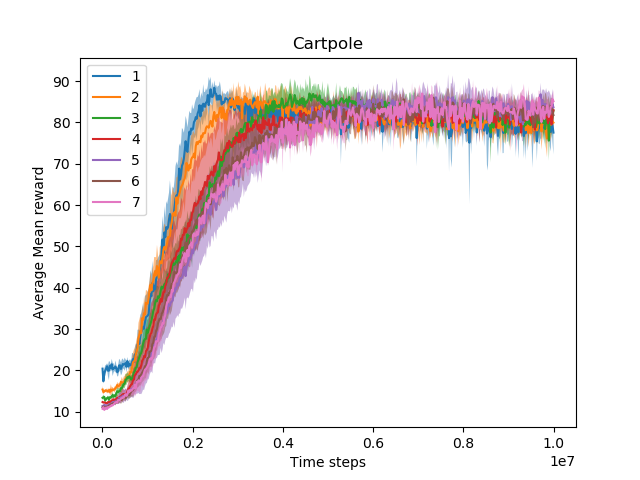
\includegraphics[width=1\textwidth,height=0.5\textheight]{../../pictures/figures/multibinary-nd-cart.png}
  \caption{Default PPO2 solving the nd cartpole problem with access to a \textit{MultiBinary} action space. Each color corresponds to a the average mean return of different, $n$, the number of repeated cart pole problems.}
\end{figure}

As mentioned in the previous section, we expected learning to become much
harder for a learner that doesn't exploit symmetries. These results suggest either of two possibilities:
that PPO2 can discover and exploit symmetries, our setting does not test what we think it does. {\color{red}so... how did we answer this???}

While investigating this further, we realised that the given action space, \textit{MultiBinary}, provies a large amount of information. We ran another test with a \textit{Discrete} action space. Where the learner gets to choose $a\in \mathbb Z_n$.
This action then gets (binary) decoded to the \textit{MultiBinary} format.

A learner that exploits the permutation symmetries in the $n$-dimensional cart pole problem should learn $n$ times quicker.
However, the cost of discovering this permutation symmetry is unknown.

\begin{figure}[h!]
\centering
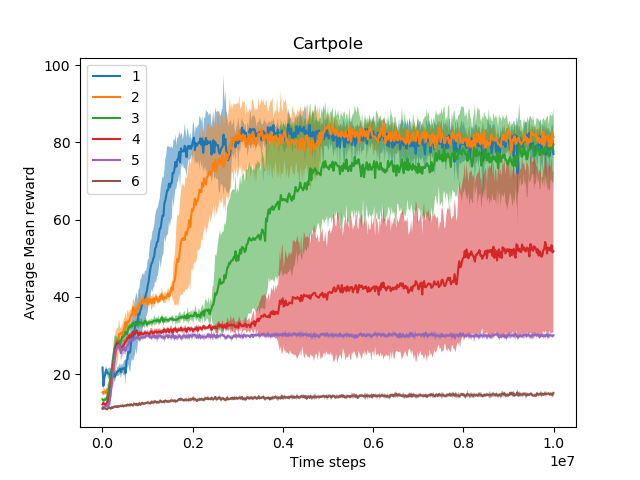
\includegraphics[width=1\textwidth,height=0.5\textheight]{../../pictures/figures/discrete-nd-cart.png}
\caption{Default PPO2 solving the nd cartpole problem with access to a \textit{Discrete} action space. Each color corresponds to a the average mean return of different, $n$, the number of repeated cart pole problems.}
\end{figure}



% It seems surprising that access to the \textit{MultiBinary} action space provides such an advantage.
% Also, it seems surprising that the an increase of 6 dimensions only results in approximately a ~2 million increase in the data required.
% Is the learner doing some sort of intelligent sharing?
% Why is it so hard for the Discrete learner? What operation does it find hard to learn. The ability to decode? $n$ bits to $2^n$ onehots?

% Also, interesting to note that the 1D learner equipped with a \textit{Discrete}
% action space achieves max performance at ~1.75 million samples, while the learner
% equipped with a \textit{MultiBinary} action space achieves max performance at ~2.25 million samples. (significant??)


Future work. The hardness of learning a binary decoder is not sufficient to explain the difference between the
\textit{Discrete} and \textit{MultiBinary} action spaces.
